\section{Binary Classification}
This section focuses on the binary discrimination between \textit{Classical} and \textit{Jazz}, which are the two largest classes in the labeled sample. Restricting the dataset to these two genres yields \(4{,}354\) observations in total. After applying the prescribed split described in Section~II, the training subset contains \(2{,}851\) tracks, including \(1{,}512\) \textit{Classical} tracks and \(1{,}339\) \textit{Jazz} tracks. In the binary response variable, \textit{Jazz} is encoded as the success category.
\subsection{Logistic regression models}
Given the nature of the problem, a logistic regression model is proposed in order to classify an observation \(x\), defined in the space of the selected system variables, into the category of interest, which has been fixed as \textit{Jazz}. Therefore, the mathematical formulation used for the model is
\begin{equation}
P(Y = 1 \mid X = x) =
\frac{\exp\left(\beta_0 + x^\top \beta\right)}
{1 + \exp\left(\beta_0 + x^\top \beta\right)}.
\label{eq:logistic_model_binary}
\end{equation}

However, the predictor space has a relatively high dimension, with \(165\) retained predictors. For this reason, several maximum-likelihood logistic regression models are compared, each imposing a different restriction on the number of retained variables. The models are defined as follows:
\begin{itemize}
    \item \textbf{Full logistic model (ModT):} includes all \(165\) retained predictors.
    \item \textbf{Mod1:} retains only predictors whose Wald p-value satisfies \(p_j < 0.05\) in ModT.
    \item \textbf{Mod2:} retains only predictors whose Wald p-value satisfies \(p_j < 0.20\) in ModT.
    \item \textbf{Stepwise logistic model (ModAIC):} selects variables by applying \texttt{stepAIC} to ModT.
\end{itemize}

This comparison makes it possible to evaluate the effect of variable selection on model complexity, numerical stability, interpretability, and predictive performance.

The relative adequacy of the reduced unpenalized logistic models with respect to the full model is assessed through likelihood-ratio tests based on deviance differences. The corresponding results are reported in Table~\ref{tab:binary_adequacy_tests}.

\begin{table}[!t]
\caption{Adequacy Tests of Reduced Logistic Models Against the Full Model}
\label{tab:binary_adequacy_tests}
\centering
\footnotesize
\begin{tabular}{lcccc}
\hline
Model & Df & Deviance & \(p\)-value & Adequate \\
\hline
\texttt{Mod1} & 107 & 256.51 & \(2.70 \times 10^{-14}\) & No \\
\texttt{Mod2} & 83 & 109.65 & 0.0267 & No \\
\texttt{ModAIC} & 74 & 37.01 & 0.9999 & Yes \\
\hline
\end{tabular}
\end{table}

The reduced models are evaluated through adequacy tests in order to determine whether a simpler specification can preserve the essential fit of the full logistic model. In logistic regression, this is assessed by comparing nested models using the difference in deviances, which measures the gain in log-likelihood obtained when moving from the reduced model to the complete model.

As shown in Fig.~\ref{tab:binary_adequacy_tests}, only the stepwise AIC model exhibits an adequate behavior. The deviance-based likelihood-ratio comparison indicates that \texttt{ModAIC} is not significantly inferior to \texttt{ModT}, suggesting that the AIC-selected model retains the essential fit of the full specification while using fewer predictors.

\subsection{Regularized Logistic Regression}

The interest of ridge regression in this study comes from the combination of a high-dimensional predictor space and residual dependence between acoustic descriptors, even after the preprocessing stage. In such a setting, an unpenalized logistic model may yield unstable coefficient estimates and may overfit the training data. Ridge regularization addresses this issue by shrinking the coefficients toward zero, which improves numerical stability and reduces the variance of the fitted classifier.

More specifically, ridge is useful here because it allows the model to keep the information carried by many correlated predictors without relying on a hard variable-selection rule. Instead of arbitrarily retaining only one variable among several related descriptors, the penalty distributes the effect more smoothly across them. For this reason, ridge is introduced as a way to control effective model complexity and to improve generalization performance in the binary classification task. The corresponding mathematical formulation is recalled in Appendix~\ref{app:skewness}, Subsection~\ref{subsec:ridge_regularization}.

In the \texttt{glmnet} algorithm, two extreme values of the regularization parameter are considered. The first one corresponds to \(\lambda = 10^{10}\), a case in which the penalization term dominates the fitting criterion. As a consequence, the coefficients associated with the predictors are strongly shrunk and approach values close to zero at the end of the training process. The second case corresponds to \(\lambda = 10^{-2}\), where the penalization is weak. In this situation, the fitted model is closer to a non-regularized logistic regression model using all retained predictors. Therefore, this configuration can be interpreted as being conceptually close to the maximum-likelihood logistic model.

Ridge regularization does not produce a single model directly, but rather a complete regularization path, corresponding to the family of fitted models obtained for different values of \(\lambda\). However, from this family of models, it is necessary to select one final specification associated with a particular value of the regularization parameter.

The method proposed for selecting this value of \(\lambda$ is 10-fold cross-validation. The training set is divided into 10 subsamples. Successively, 9 of them are used to fit the ridge model, while the remaining subsample is used to evaluate the prediction error. This procedure is repeated until each fold has been used once as the validation sample.

For each value of \(\lambda$ in the grid, the prediction errors obtained over the 10 folds are averaged. The final retained value is \texttt{lambda.min}, that is, the value of \(\lambda$ that minimizes the mean cross-validation error. This leads to the final regularized model used for the binary classification task.

From the cross-validation results, displayed in Fig.~\ref{fig:ridge_cv_plot}, it can be observed that when \(\lambda$ is very large, the penalization is too strong. As a consequence, the model becomes highly constrained and the binomial deviance remains high. Conversely, as \(\lambda$ decreases, the model gains flexibility and the error decreases, indicating that, for the training data, an excessively strong penalization deteriorates the fit.

This suggests that, in order to minimize the binomial deviance, the model needs to remain relatively close to the non-regularized logistic regression. However, since ridge regression retains the \(165\) predictors and does not perform hard variable selection, the signal is still distributed across many predictors, including weak or redundant ones.

\begin{figure}[!t]
\centering
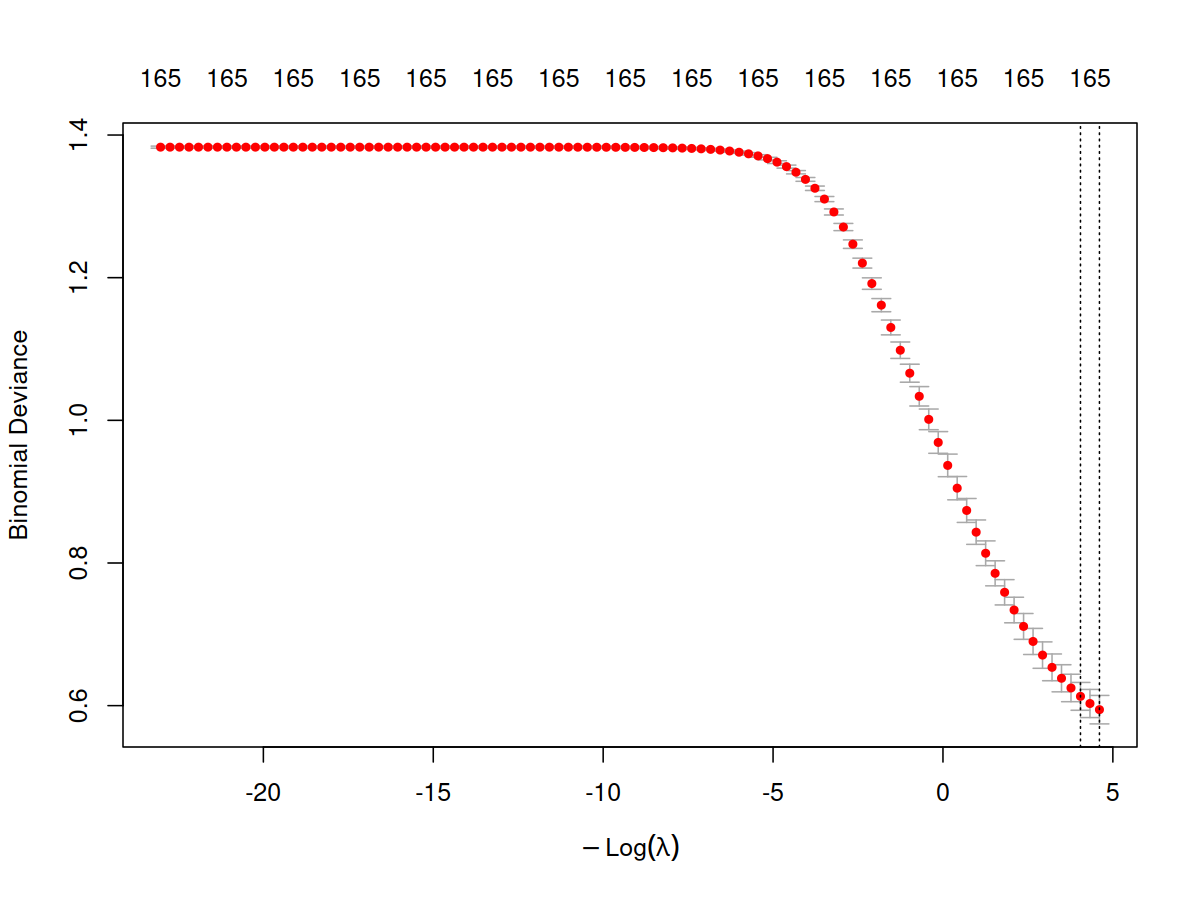
\includegraphics[width=\columnwidth]{../output/part2/ridge_cv/ridge_cv_plot.png}
\caption{Ten-fold cross-validation curve used to select the ridge regularization parameter. The retained value corresponds to the minimizer of the mean binomial deviance.}
\label{fig:ridge_cv_plot}
\end{figure}

\subsection{Summary of Binary Classification Results}

Table~\ref{tab:model_comparison} summarizes the main performance indicators for all five models evaluated on the test set. The AUC values are uniformly high, reflecting the strong linear separability of \textit{Classical} and \textit{Jazz} in the acoustic feature space. All models outperform the random baseline by a large margin.

\begin{table}[!t]
\centering
\caption{Performance summary for all binary classifiers on the test set.}
\label{tab:model_comparison}
\scriptsize
\resizebox{\columnwidth}{!}{%
\begin{tabular}{lcccc}
\toprule
Model & AUC (test) & Accuracy & Error rate & \# Variables \\
\midrule
ModT   & 0.9627 & 0.9095 & 0.0905 & 165 \\
Mod1   & 0.9543 & 0.8902 & 0.1098 & 58 \\
Mod2   & 0.9605 & 0.9022 & 0.0978 & 82 \\
ModAIC & 0.9629 & 0.9082 & 0.0918 & 91 \\
Ridge  & 0.9414 & 0.8842 & 0.1158 & 165 \\
\bottomrule
\end{tabular}}
\end{table}

The ridge model achieves a competitive AUC despite using a soft rather than hard variable-selection strategy, confirming that regularization provides a meaningful alternative to coefficient-wise significance thresholding when many predictors are correlated.

Based on the empirical evaluation on the test set, \textbf{ModAIC} achieves the highest AUC (\(0.9629\)) and the second highest accuracy (\(0.9082\)). It also provides a more parsimonious representation than the full and ridge models by reducing the active predictor space from \(165\) to \(91\) variables. Consequently, \textbf{ModAIC} is selected as the final binary classifier for this task. The genre predictions for the unlabeled holdout file were generated using this model and saved to the corresponding submission file.
